\chapter{Arbeitsgrundlagen}
% ==================================================================
\setcounter{page}{1} \thispagestyle{fancy} 
% ==================================================================
\section{Das Röntgen-Spektrum}
Wenn schnelle Elektronen auf Materie treffen, dann entstehen Röntgenstrahlen. Eine Röntgen-Röhre besteht aus (siehe Abbildung \ref{fig:roentgen_roehre}):
\begin{itemize}
\item[\textbf{K}] \textbf{Glühkathode}
\item[\textbf{A}] \textbf{massive Anode} (je nach Verwendungszweck ein Metall mittlerer bis hoher Ordnungszahl)
\item[\textbf{U}] \textbf{Hochspannung} (Bereich von $10kV$ bis zu einigen $100kV$)
\end{itemize}
Die Glühkathode und die massive Anode sind dabei von einem evakuierten Glaskolben umschlossen. Von der Kathode emittieren Elektronen, welche von der angelegten Hochspannung beschleunigt werden. Mit einer fokussierten Energie von ungefähr $E_{k} = e*U$ prallen diese dann auf die Anode. In einer Schicht von wenigen $\mu m$ Dicke verlieren die Elektronen ihre Energie durch eine Kette von Stoßprozessen. Hauptsächlich durch Anregung und Ionisation der Metallatome ($>99\%$). Diese Energie wird in Wärme umgewandelt, weshalb die Anoden rotiert oder mit Wasser gekühlt werden müssen. Somit bleibt nur noch ein kleiner Rest übrig ($<1\%$), welcher in Röntgenstrahlung umgesetzt wird. Die resultierende Strahlung entspricht einer isotropen Strahlung (\textit{Isotropie}\footnote{\textit{kursiv} geschriebene Begriffe sind im Kapitel \nameref{chap:begriffsexplikation} genauer erläutert}), was eine Abschirmung erfordert. Die Nutzstrahlung wird mit einem Bleikollimator ausgeblendet. Die Anode ist abgeschrägt und der Kolben mit einem Fenster aus dünnerem Glas oder Beryllium versehen, damit die Absorptionen  niedrig gehalten werden können.
\begin{figure}[h]
\centering
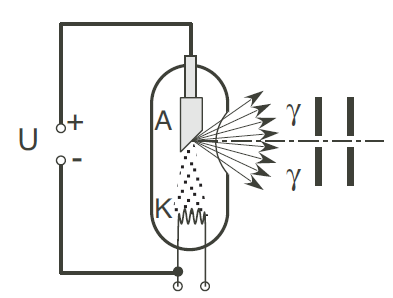
\includegraphics[scale=1.5]{Bilder/roentgen_roehre.png} 
\label{fig:roentgen_roehre}
\caption{Röntgen-Röhre}
\end{figure}
\newpage

\begin{wrapfigure}{r}{0.5\textwidth}
\centering
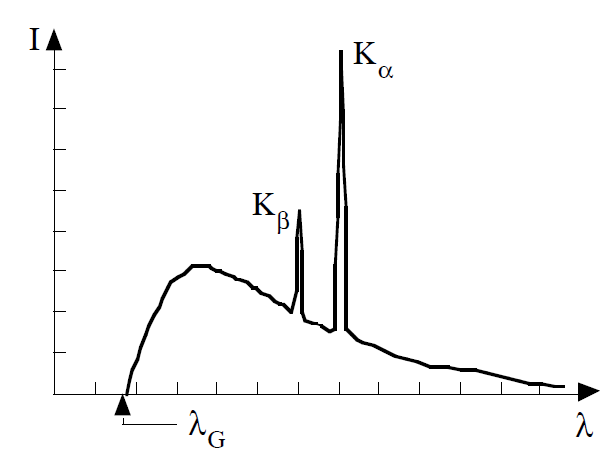
\includegraphics[width=0.48\textwidth]{Bilder/roentgen_spektrum.png}
\caption[Röntgenspektrum]{Röntgenspektrum: \textbf{I} steht für die Intensität und $\lambda$ für die Wellenlänge.}
\vspace{-1.5cm}
\label{fig:roentgenspektrum}
\end{wrapfigure}

Aus der Abbildung \ref{fig:roentgenspektrum} kann entnommen werden, dass das Röntgenspektrum aus zwei Komponenten besteht:\\
\begin{itemize}
\item \textbf{Bremskontinuum}: Es weisst eine unspezifische Form auf und beginnt am kurzweiligen Ende bei einem von der angelegten Spannung abhängigen Punkt ($\lambda_{G}$)\\
\item \textbf{Röntgenlinien}: ($K_{\alpha}$ \& $K_{\beta}$) Diese sind charakteristisch für das Anodenmaterial und hängen nicht von der Spannung ab\\
\end{itemize}


\subsection{Die Bremsstrahlung}
\begin{wrapfigure}{l}{0.5\textwidth}
\centering
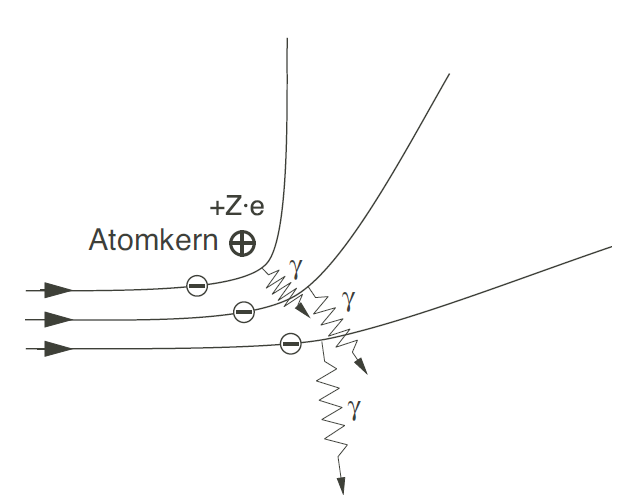
\includegraphics[width=0.48\textwidth]{Bilder/bremsstrahlung.png} 
\caption{Entstehung der Bremsstrahlung}
\vspace{-1.5cm}
\label{fig:bremsstrahlung}
\end{wrapfigure}
Wenn Elektronen in das Coulombfeld im Kern eines Atoms eindringen, dann entsteht die Bremsstrahlung. Dabei wird auf das Elektron durch die Coulombkraft eine Zentralbeschleunigung gegen den Kern (\textit{Zentripetalkraft}) ausgeübt, wodurch es auf einer Hyperbelbahn am Kern vorbeifliegt. Da das Elektron aber eine elektromagnetische Strahlung aussendet, verlässt es das Coulombfeld mit Energieverlust.\\[0.5cm]
\textbf{Wichtig}: Dieser Energieverlust, resp. diese Bremsung des Elektrons wird durch genau diese elektromagnetische Abstrahlung des Elektrons kausiert, nicht umgekehrt!
\\[0.5cm]
Wegen der hohen Geschwindigkeit der Elektronen dauert die Beschleunigung nur eine sehr kurze Zeit, weshalb eine \textit{aperiodische} Stosswelle emittiert. Dessen Frequenzspektrum entspricht einem Kontinuum, welches je kürzer die Abstrahlung, umso breiter ist und sich bis zu beliebig hohen Frequenzen erstreckt. Bei der Ablenkung des Elektron wird nach der Quantentheorie der Strahlung ein Photon $\gamma$ (siehe Abbildung \ref{fig:bremsstrahlung}) emittiert. Bei dieser Photonenemission spielt sich ein Elementarprozess ab, bei dem die Energie und der Impuls erhalten bleibt, wobei die Energiezustände kontinuierlich sind. Weil der Kern sehr schwer ist, nimmt er praktisch keine Energie auf, weshalb sich die Energie des einfallenden Elektrons $E_{e}$ rein zufällig auf das Elektron und das Photon teilt. Die Energie des Photons $E_{\gamma},max$ kann somit höchstens gleich der Energie des Elektrons $E_{e}$ werden. Daraus schliesst sich, dass das Bremskontinuum bei der Grenzfrequenz $f_{G} = \dfrac{E_{e}}{h}$ und somit bei der Wellenlänge $\lambda_{G} = \dfrac{h*c}{E_{e}}$ abbrechen muss.
Die Bremsstrahlung hat die Grenze bei:\\
\begin{equation}
\Large
E_{\lambda,max}=e*U,\; bzw. \; \lambda_{G}=\dfrac{h*c}{e*U}
\end{equation}
\newpage

\subsection{Die charakteristische Strahlung}
\begin{wrapfigure}{r}{0.5\textwidth}
\centering
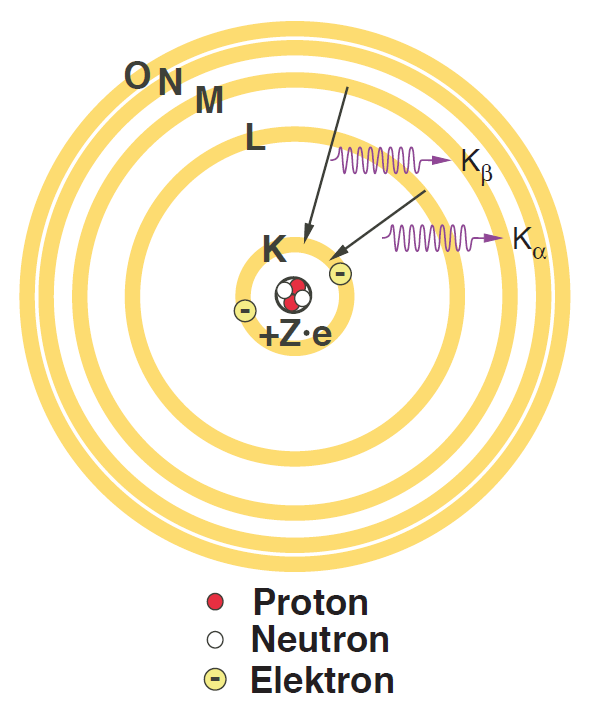
\includegraphics[width=0.48\textwidth]{Bilder/atommodell.png} 
\caption{Entstehung der charakteristischer Strahlung}
\vspace{-6cm}
\label{fig:charStrahlung}
\end{wrapfigure}
Diese Strahlung entsteht, wenn beim Elektronenübergang in der kernnahen Atomhülle des Anodenmaterials ein Photon emittiert wird. In der Abbildung \ref{fig:charStrahlung} sind diese Übergänge mit der daraus resultierenden Strahlung illustriert:
\\[0.5cm]
\begin{tabular}{llll}
L-Schale & $\rightarrow$ & K-Schale & $K_{\alpha}$-Strahlung \\ 
M-Schale & $\rightarrow$ & K-Schale & $K_{\beta}$-Strahlung \\ 
M-, N-, O-Schale & $\rightarrow$ & L-Schale & L-Strahlung \\ 
\multicolumn{4}{l}{usw.} \\ 
\end{tabular}
\\[0.5cm]
Solche Übergänge sind nur möglich, wenn zuvor ein Elektron aus der dementsprechenden Schale \glqq herausgeschlagen\grqq\; wurde. Dies geschieht entweder durch einen Elektronenstoss (Stossionisation), oder durch Absorption von Röntgen-Strahlung (Photoionisation).\\
\vspace*{3cm}
\section{Beugung von Röntgen-Strahlung an Kristallen, Röntgen-Spektrometer}
